\section{Конструкторская часть}	
	\subsection{Use-Case диаграмма}
	На рисунках \ref{fig2:image}-\ref{fig4:image} приведены диаграммы вариантов использования для каждого актора, полная схема находится в приложении.
	
	\begin{figure}[ph!]
		\centering
		\begin{center}
			{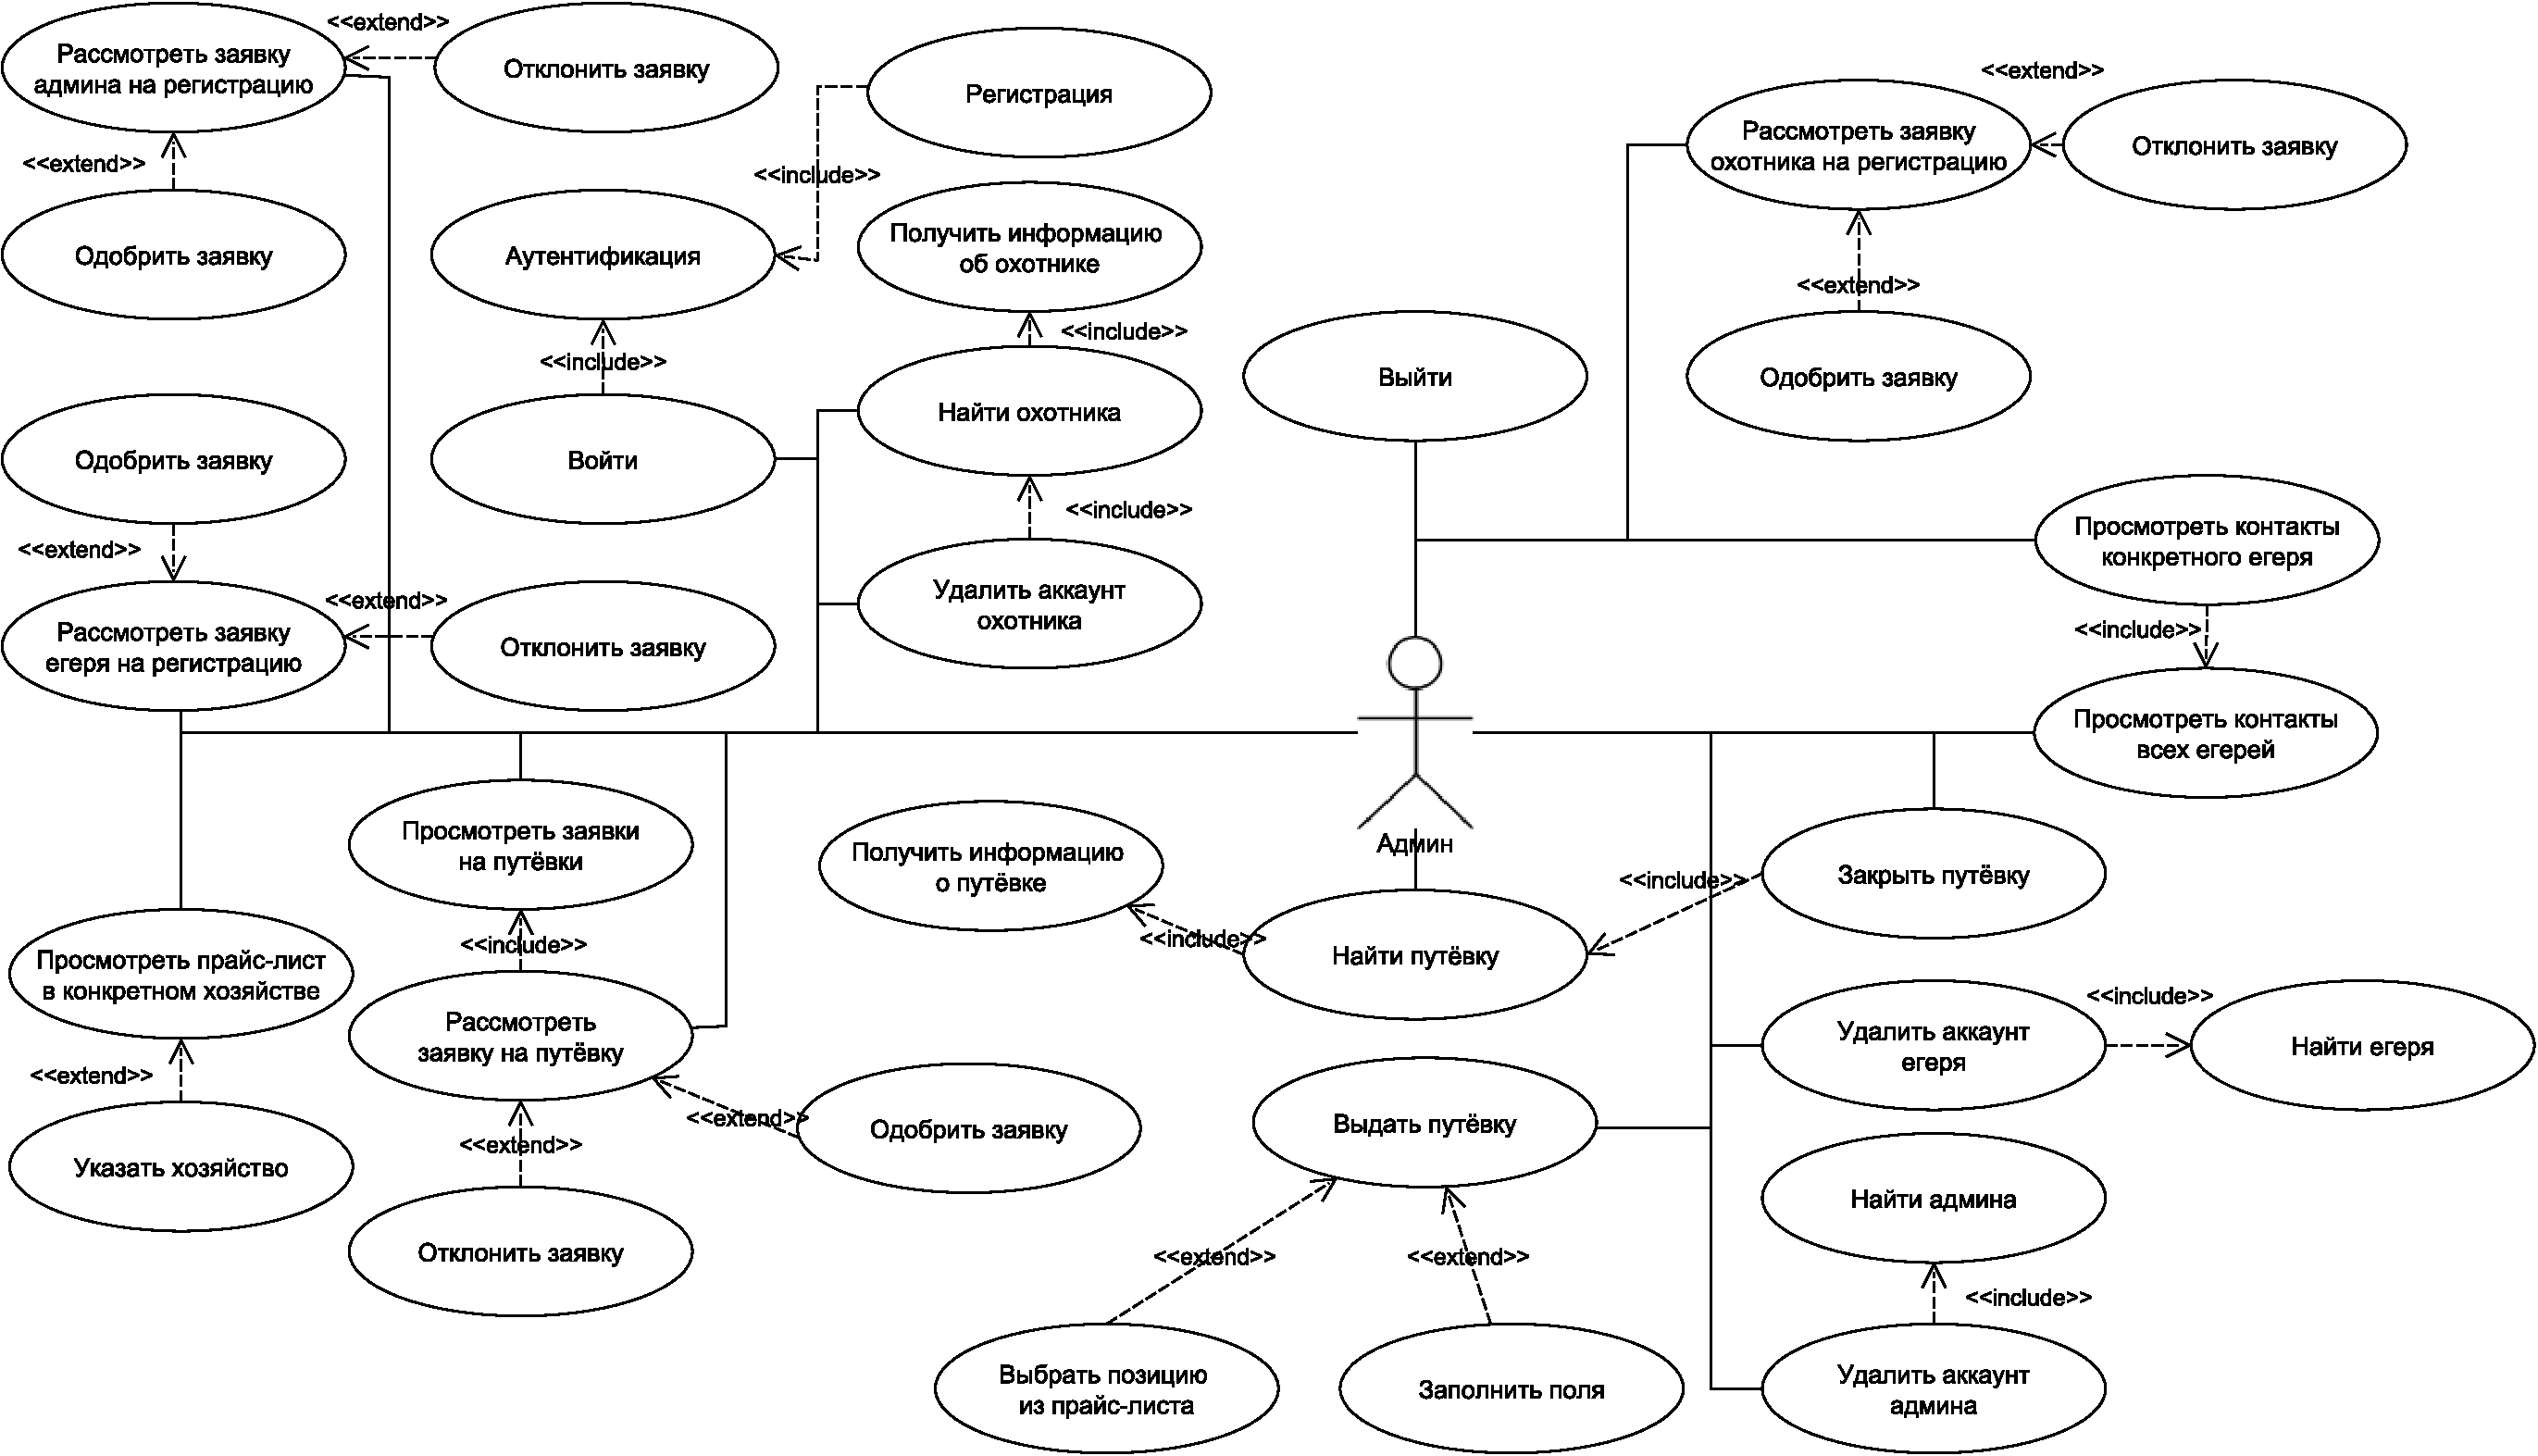
\includegraphics[scale=0.44, angle=90]{schemes/use-case_admin.pdf}}
			\caption{ER-диаграмма сущностей (администратор)}
			\label{fig2:image}
		\end{center}
	\end{figure}

	\begin{figure}[ph!]
		\centering
		\begin{center}
			{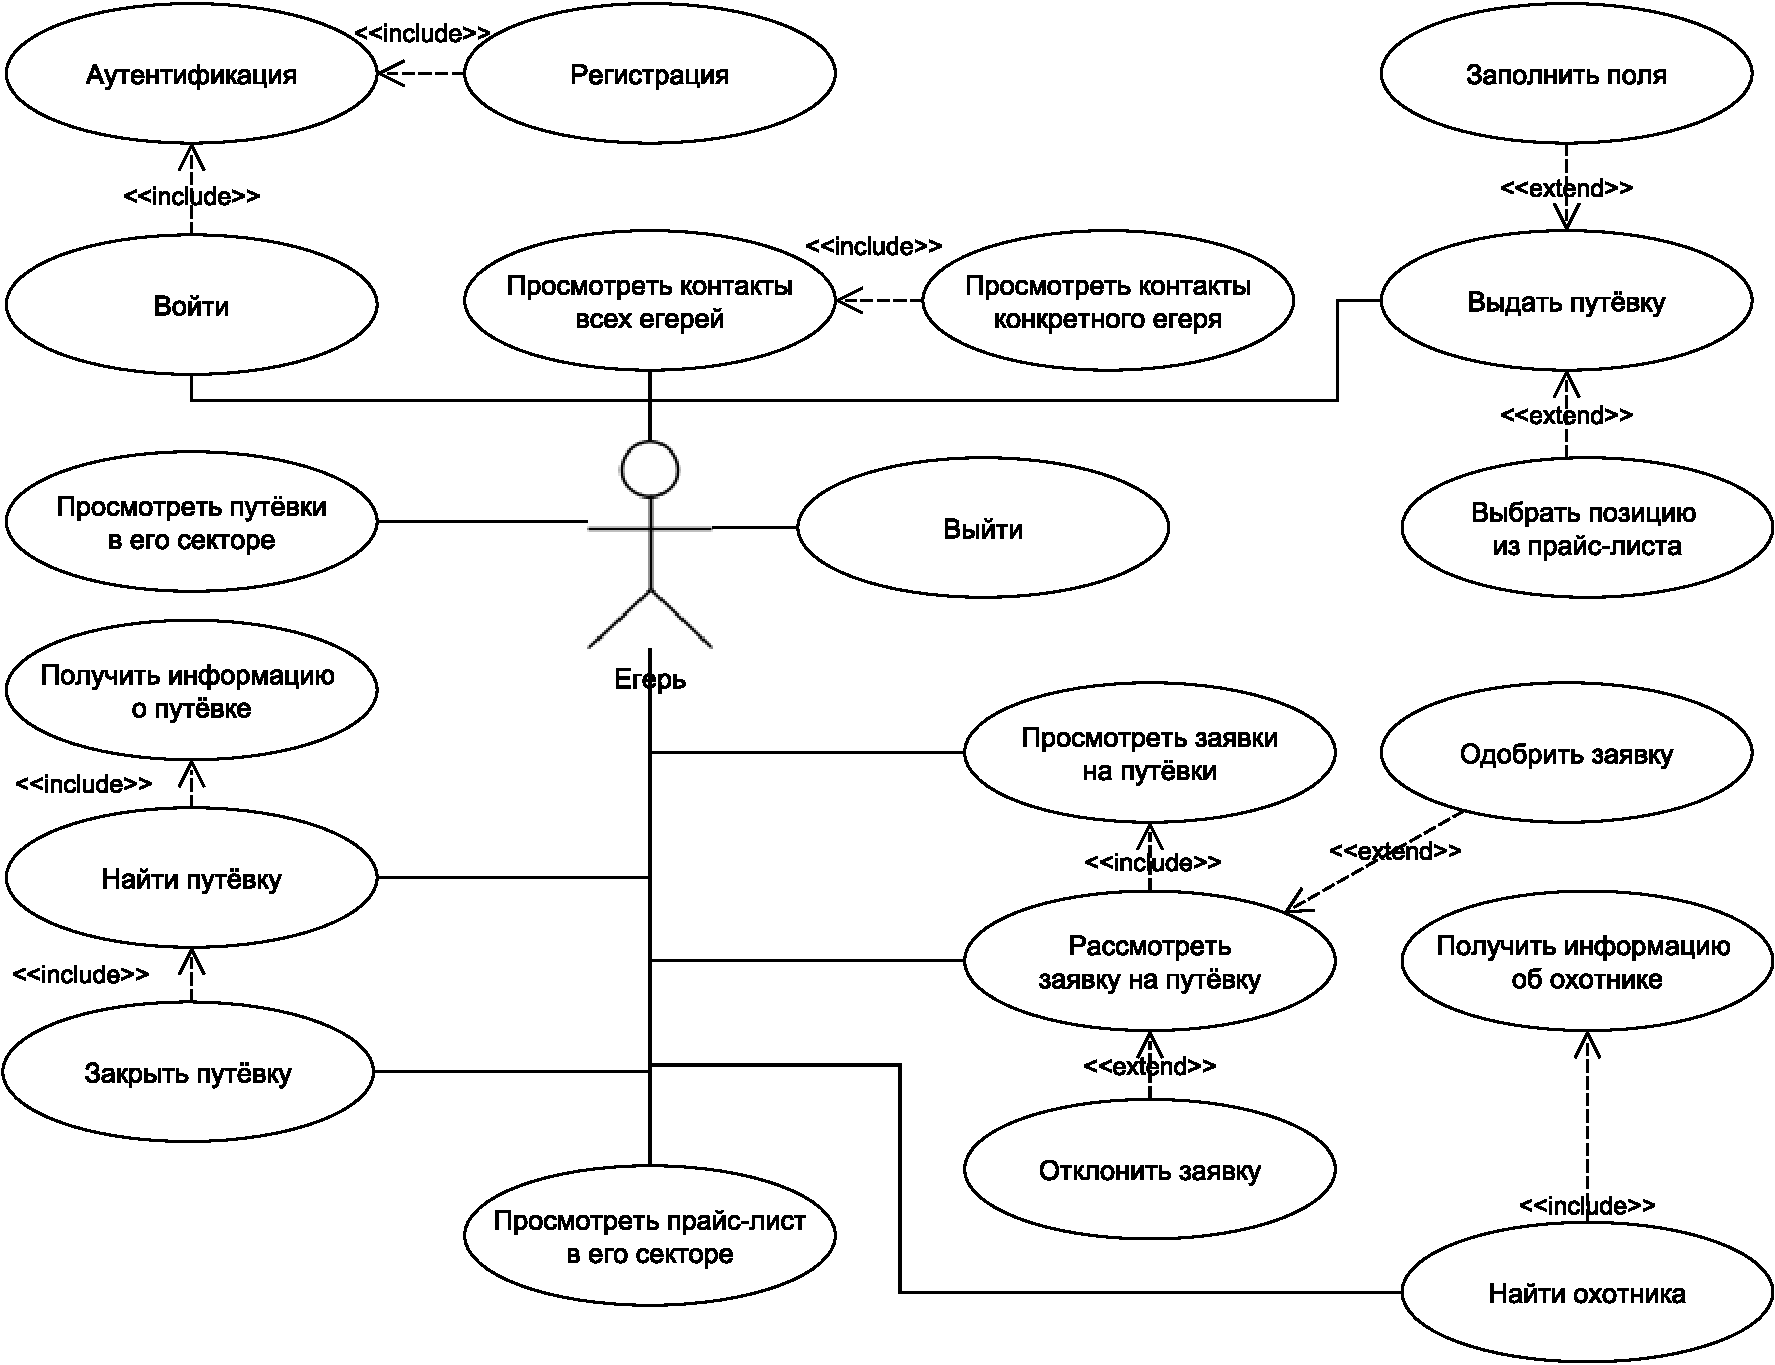
\includegraphics[scale=0.45]{schemes/use-case_huntsman.pdf}}
			\caption{ER-диаграмма сущностей (егерь)}
			\label{fig3:image}
		\end{center}
	\end{figure}

	\begin{figure}[ph!]
		\centering
		\begin{center}
			{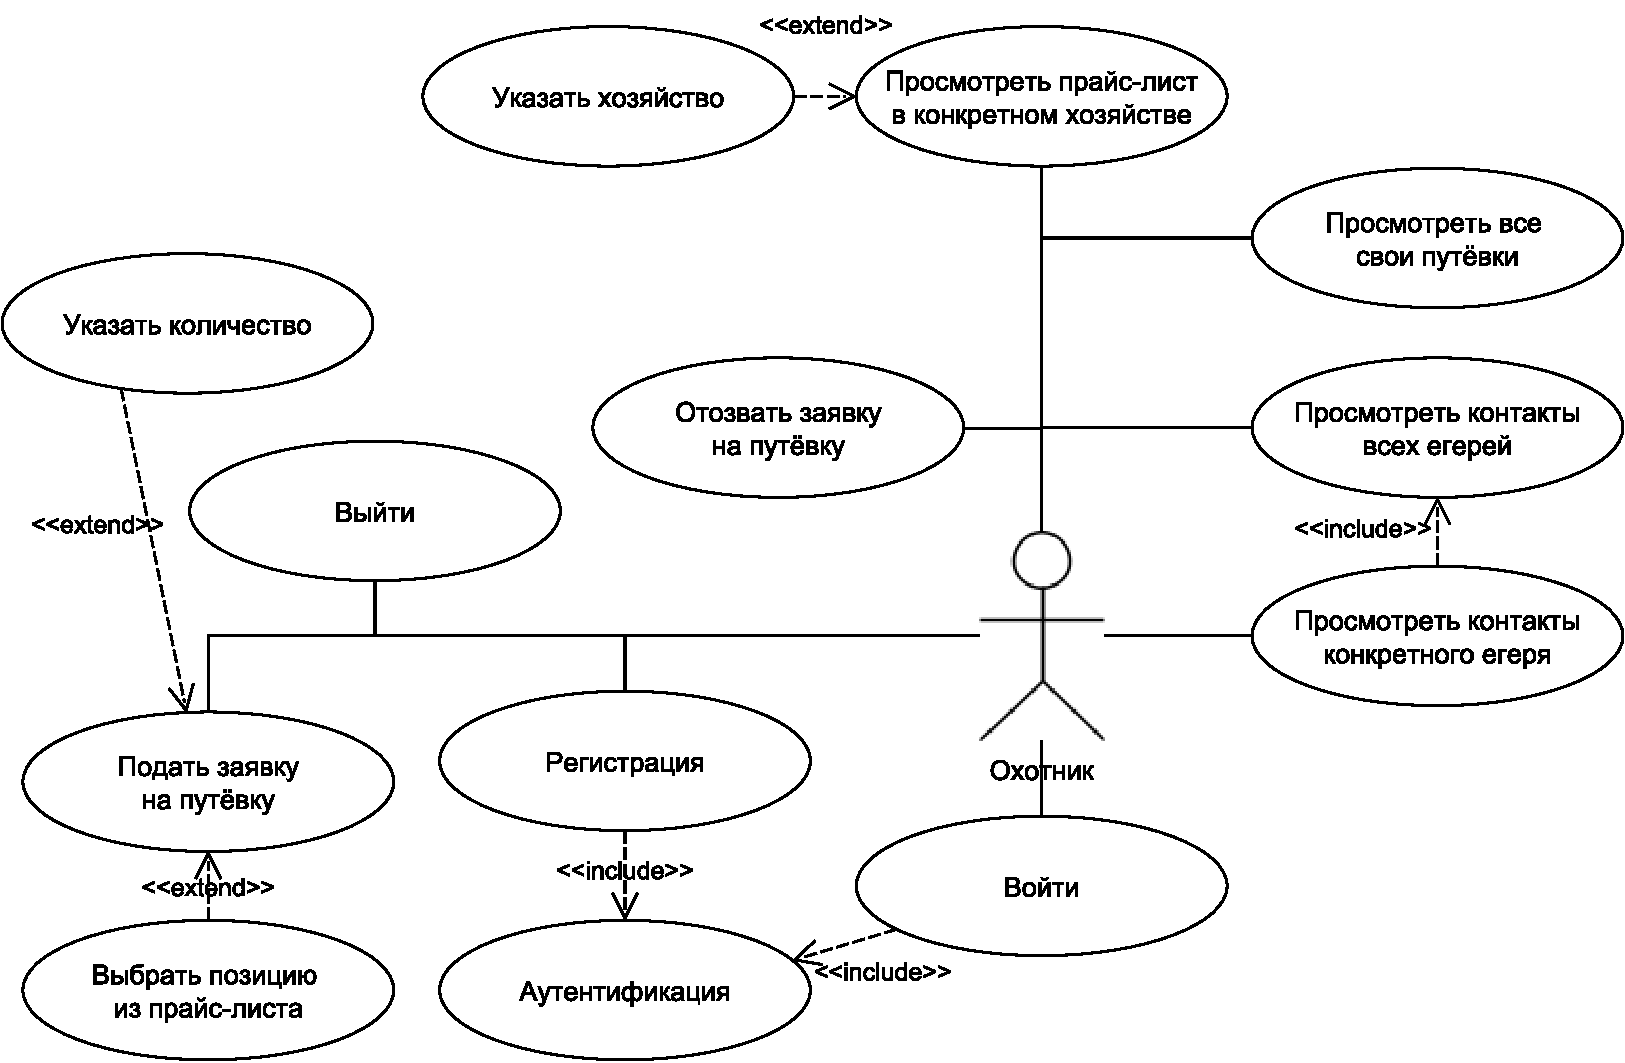
\includegraphics[scale=0.45]{schemes/use-case_hunter.pdf}}
			\caption{ER-диаграмма сущностей (охотник)}
			\label{fig4:image}
		\end{center}
	\end{figure}
	
	\newpage
	
	\subsection{ER-диаграмма сущностей БД}
	На рисунке \ref{fig5:image} приведена ER-диаграмма базы данных, на которой также указываются связи, поля таблиц и ключи.
	
	\begin{figure}[ph!]
		\centering
		\begin{center}
			{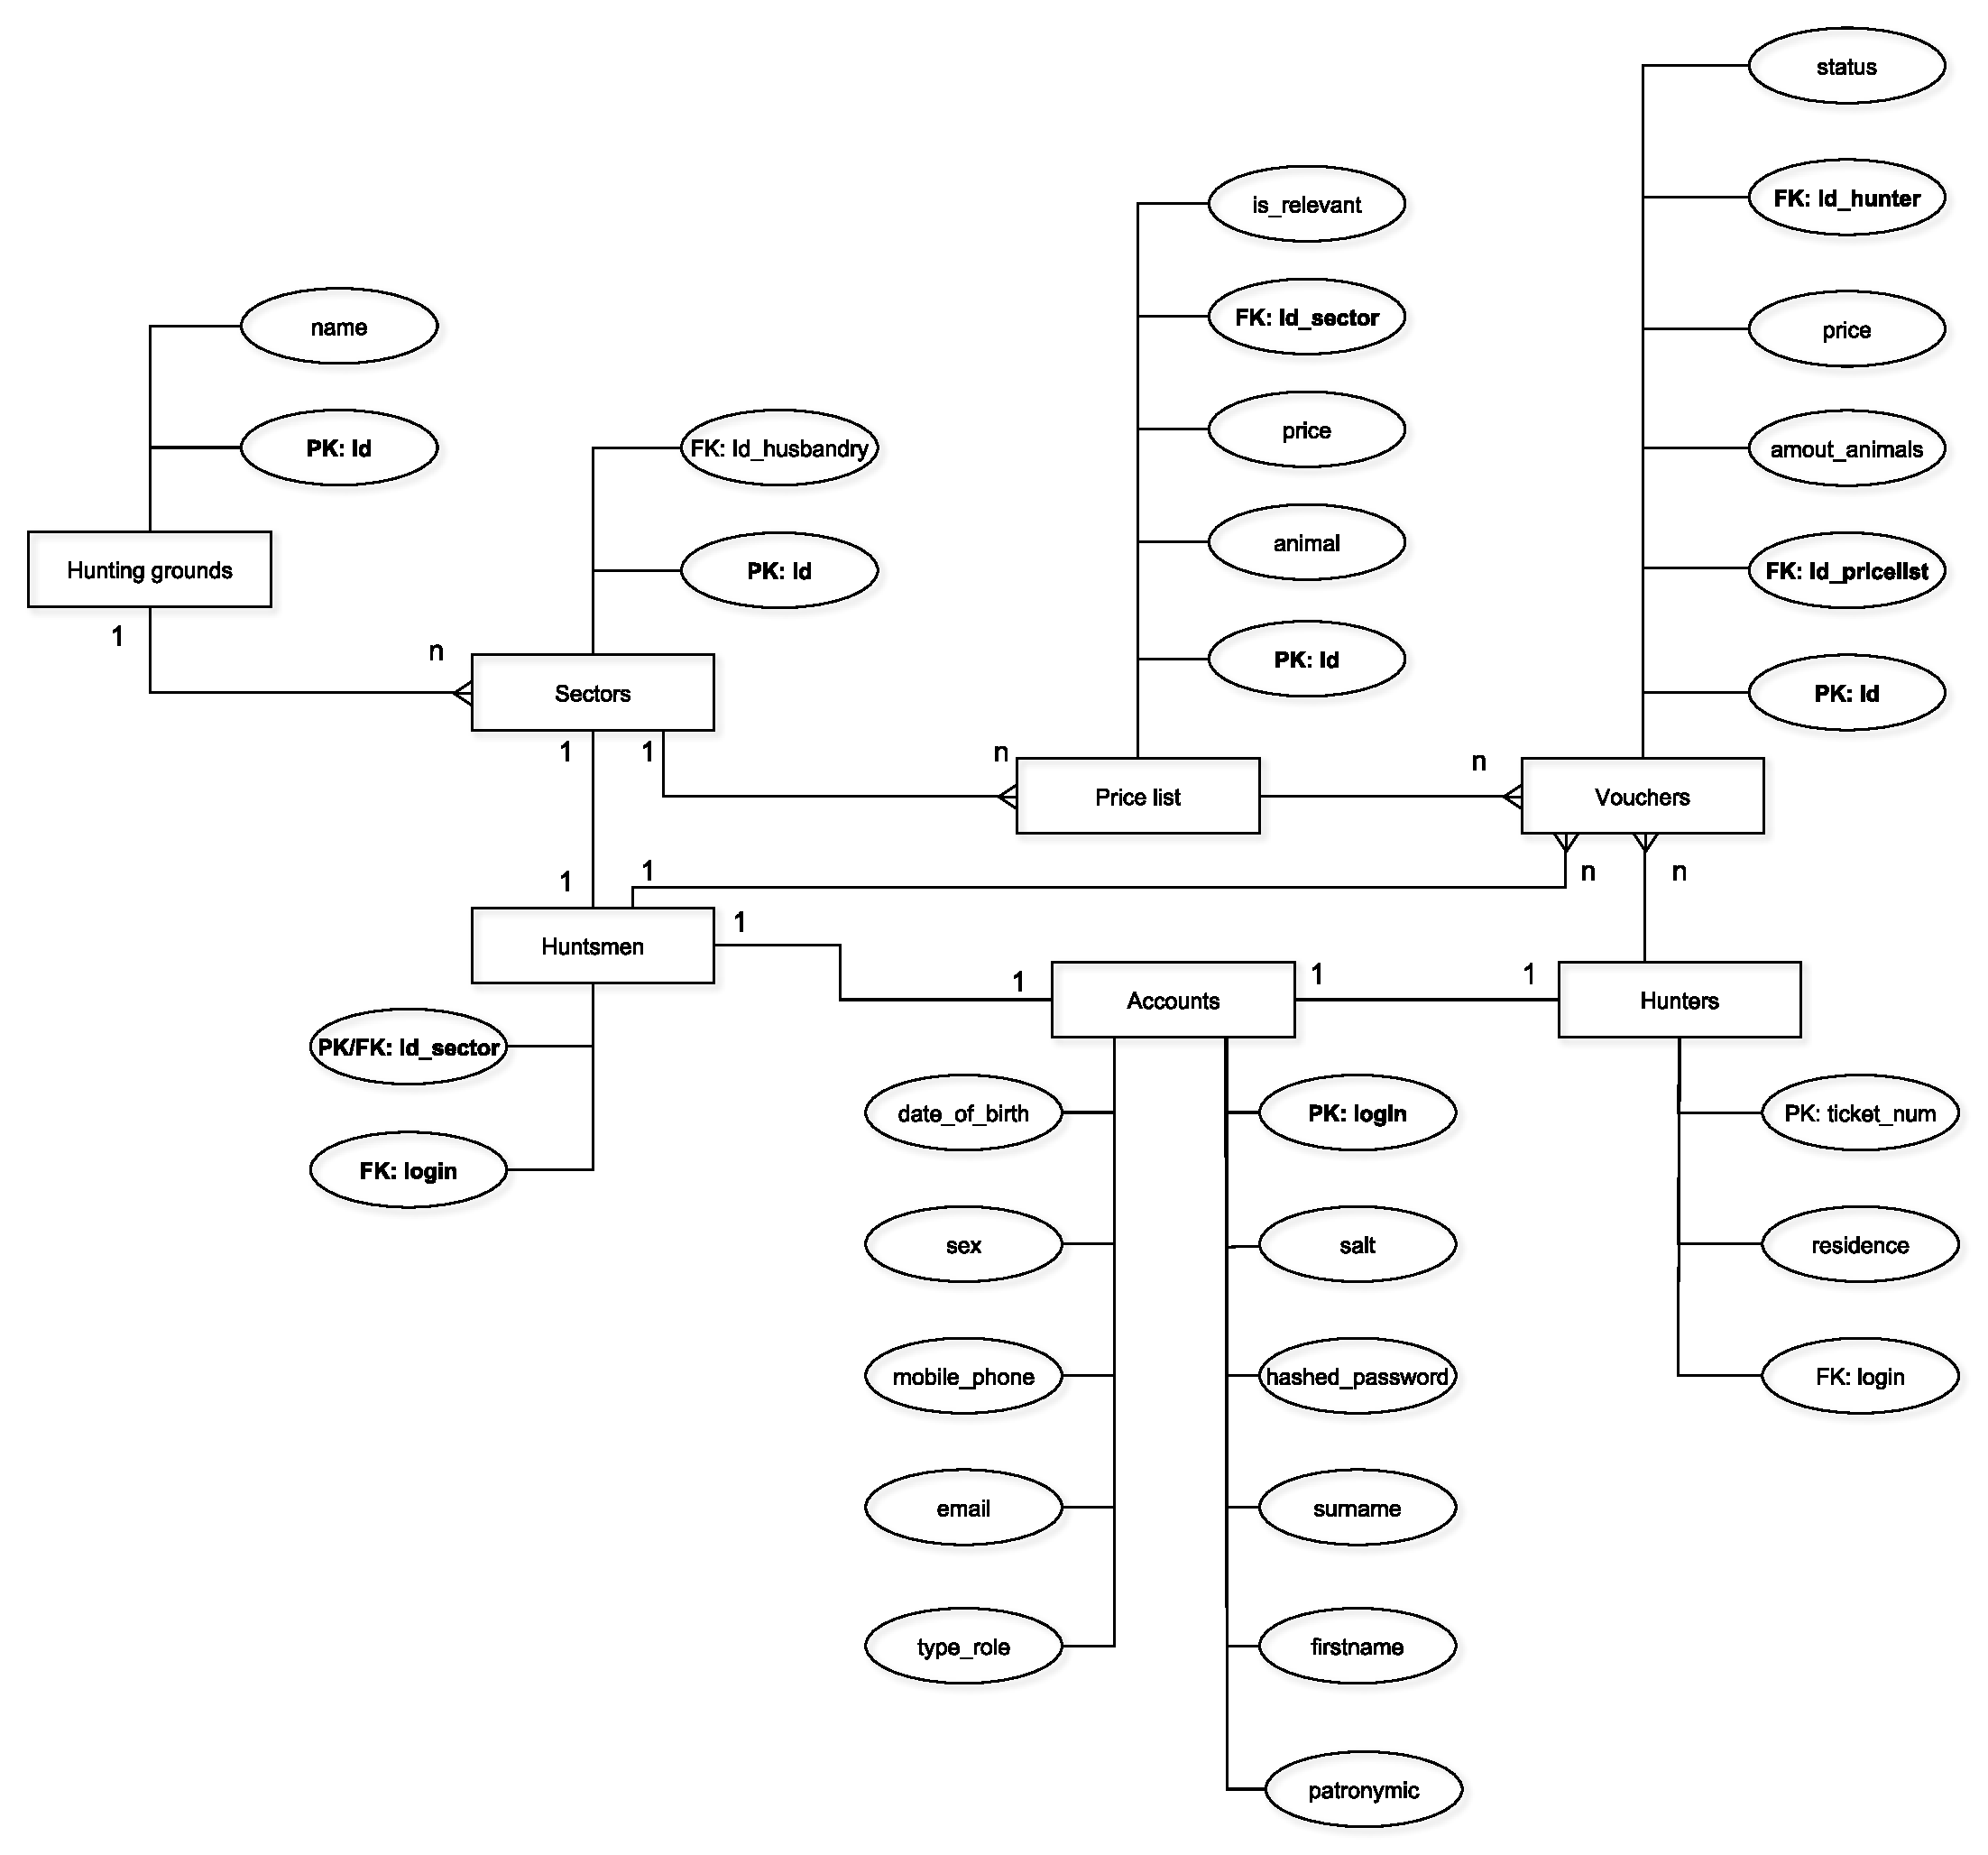
\includegraphics[scale=0.47]{schemes/ERclassic.pdf}}
			\caption{ER-диаграмма сущностей}
			\label{fig5:image}
		\end{center}
	\end{figure}

	База данных должна содержать таблицы, поля и назначение которых описаны в таблицах 
	\ref{hgtable}-\ref{vouchers_table}.
	
	\begin{table}[h] 
		\begin{center}
			\caption{HuntingGrounds (таблица хозяйств)}
			\label{hgtable}
			\begin{tabular}{| c | l |}
				\hline
				\textbf{Атрибут} 	& \textbf{Значение} \\
				\hline
				Id 					&	Идентификатор, PK \\ 
				\hline
				GroundName 			&	Название \\ 
				\hline
			\end{tabular}
		\end{center}
	\end{table}

	\begin{table}[h] 
		\begin{center}
			\caption{Sectors (таблица секторов)}
			\label{sec_table}
			\begin{tabular}{| c | l |}
				\hline
				\textbf{Атрибут} 	& \textbf{Значение} \\
				\hline
				Id 					&	Идентификатор, PK \\ 
				\hline
				IdHusbandry 			&	Идентификатор хозяйства,  \\ 
				& в состав которого входит сектор, FK \\
				\hline
			\end{tabular}
		\end{center}
	\end{table}

	\begin{table}[pt!]
		\begin{center}
			\caption{Accounts (таблица аккаунтов)}
			\label{acc_table}
			\begin{tabular}{| c | l |}
				\hline
				\textbf{Атрибут} 	& \textbf{Значение} \\
				\hline
				Login 				&	Логин, PK \\ 
				\hline
				Salt 				&	Соль  \\ 
				\hline
				HashedPassword 		&	Хэшированный пароль \\ 
				\hline
				Surname 			&	Фамилия \\ 
				\hline
				Firstname 			&	Имя \\ 
				\hline
				Patronymic 			&	Отчество \\ 
				\hline
				DateOfBirth 		&	Дата рождения \\ 
				\hline
				Sex 				&	Пол \\ 
				\hline
				MobilePhone 		&	Мобильный телефон \\ 
				\hline
				Email 				&	Электронная почта \\ 
				\hline
				TypeRole 			&	Роль \\ 
				\hline
			\end{tabular}
		\end{center}
	\end{table}

	Для обеспечение безопасности используются хэширование паролей, и в базе данных в таблице \ref{acc_table} хранится только соль и хэшированный пароль.\\

	\begin{table}[pt!] 
		\begin{center}
			\caption{Huntsmen (таблица егерей)}
			\label{huntsmen_table}
			\begin{tabular}{| c | l |}
				\hline
				\textbf{Атрибут} 	& \textbf{Значение} \\
				\hline
				Id 					&	Идентификатор сектора, за которым \\
									& 	закреплён егерь, PK, FK \\
				\hline
				Login	 			&	Логин, FK \\ 
				\hline
			\end{tabular}
		\end{center}
	\end{table}

	\begin{table}[pt!] 
		\begin{center}
			\caption{Hunters (таблица охотников)}
			\label{hunters_table}
			\begin{tabular}{| c | l |}
				\hline
				\textbf{Атрибут} 	& \textbf{Значение} \\
				\hline
				TicketNum 			&	Номер охотничьего билета, PK\\
				\hline
				Residence			& 	Адрес прописки \\
				\hline
				Login	 			&	Логин, FK \\ 
				\hline
			\end{tabular}
		\end{center}
	\end{table}

	\begin{table}[pt!]
		\begin{center}
			\caption{PriceList (таблица цен на путёвки)}
			\label{price_table}
			\begin{tabular}{| c | l |}
				\hline
				\textbf{Атрибут} 	& \textbf{Значение} \\
				\hline
				Id 					&	Идентификатор, PK\\
				\hline
				Animal				& 	Название животного \\
				\hline
				Price	 			&	Цена \\ 
				\hline
				IsRelevant	 		&	Флаг актуальности \\ 
				\hline
				IdSector	 		&	Идентификатор сектора, за которым \\
									& 	закреплена позиция, FK \\
				\hline
			\end{tabular}
		\end{center}
	\end{table}

	\begin{table}[pt!] 
		\begin{center}
			\caption{Vouchers (таблица путёвок)}
			\label{vouchers_table}
			\begin{tabular}{| c | l |}
				\hline
				\textbf{Атрибут} 	& \textbf{Значение} \\
				\hline
				Id 					&	Идентификатор, PK\\
				\hline
				AmountAnimals		& 	Количество животных \\
				\hline
				Price	 			&	Цена \\ 
				\hline
				IdHunter	 		&	Идентификатор владельца-охотника, FK \\ 
				\hline
				IdPricelist	 		&	Идентификатор позиции из перечня цен, FK \\
				\hline
				Status				& 	Статус (ждёт решения/одобрено) \\
				\hline
			\end{tabular}
		\end{center}
	\end{table}

	\subsection{Архитектура приложения. Модель MVC}
	Этот шаблон проектирования предполагает разделение на три отдельных компонента: Модель (Model), Представление (View) и Контроллер (Controller). Это позволяет производить модификации какого-либо компонента независимо от других. \cite{mvc} 
	
	\textbf{Model} - компонент бизнес-логики приложения, предоставляет данные и методы работы с ними.
	
	\textbf{View} - компонент, который отвечает за взаимодействие с пользователем, необходим для отображения данных, полученных в результате работы модели.
	
	\textbf{Controller} отвечает за обработку действий пользователя, перенаправляет данные от пользователя к модели и наоборот.\\
	
	\subsection{Вывод}




	
	